\begin{frame}{}
\begin{large}
\begin{center}
B.2 Recursive Utilities and Epstein-Zin Preferences
\end{center}
\end{large}
\end{frame}


\begin{frame}{}
\begin{footnotesize}
\begin{itemize}
	\item Given the problems of the consumption-based models, one has questioned the utility function [e.g. \href{http://faculty.chicagobooth.edu/john.cochrane/research/papers/financial_and_real_proofs_aug_07.pdf}{Cochrane 2007, p.270}].
	\item Functional form is not really an issue: in the time-separable framework, linearized and non-linearized models behave relatively similarly.

	\begin{tiny}
	[Utility functions are monotonously $\nnearrow$ with negative second order derivatives.]	\end{tiny}
	\item What about the arguments of the utility function?
	
	{\bf Idea}: The marginal utility of consumption may not depend only on today's consumption.
	%\item For this, the utility function must be non-separable.
	%Indeed, if $u(c,x)=v(c)+w(x)$, then $\partial u(c,x)/\partial c = v'(c)$ and $x$ does not matter for asset pricing.
	
	\item Pricing implications are very different when the marginal utility of consumption depends past or (expected) future consumption.
\end{itemize}
\end{footnotesize}
\end{frame}



\begin{frame}{}
\begin{footnotesize}
\begin{defn}[Expected Utility Time-Separable Preferences]\label{def:EUTSpref}
In the context of {\color{blue}expected utility time-separable preferences}, the intertemporal utility $U_t$ is defined as:
$$
U_t = \mathbb{E}_t\left(\sum_{i=0}^{\infty} \delta^{i}u(C_{t+i})\right),
$$
or, equivalently, as:
$$
U_t = u(C_t) + \delta \mathbb{E}_t\left(U_{t+1}\right).
$$
\end{defn}

\vspace{.5cm}
Implications of expected utility time-separable preferences:
	\begin{itemize}
		\item No premium for early resolution of uncertainty.
		
		As of date $t$, the promise to know $C_{t+h}$ at date $t+1$ has no value.
		\item No utility effect of potential autocorrelation in $C_t$:
		
		Each stream of consumption intervenes independently from the others in the utility computation.
	\end{itemize}
\end{footnotesize}
\end{frame}



\begin{frame}{}
\begin{footnotesize}
\begin{itemize}
	\item What does {\color{blue}non-separability over time} means?
	
	That the marginal utility of today's consumption depends on past consumption.
	
	%\textit{"Yesterday's pizza lowers the marginal utility for another pizza today."}
	
	In other words, 	what you consumed yesterday can have an impact on how you feel about more consumption today.

	
	\item Example: {\color{blue}Habit formation} [\href{http://faculty.chicagobooth.edu/john.cochrane/research/papers/campbell_cochrane_by_force_of_habit_(jpe).pdf}{Campbell and Cochrane (1999)}]
	\begin{equation}\label{eq:Uhabit_nonstoch}
	U_t = \sum_{s=t}^{\infty} \delta^{s-t} u(C_s - X_s) \quad where \quad X_t = \rho X_{t-1} + \lambda C_t.
	\end{equation}
	
	\item The date-$t$ utility associated with a level of consumption $C_t$, that is $u(C_t - X_t)$, is lower is you already had a high level of consumption at date $t-1$ (high $X_t$).
	$$
	U_t = \sum_{h=0}^{\infty} \delta^{h}u\left(C_{t+h} - \lambda \sum_{j=0}^\infty \rho^j C_{t+h-j}\right).
	$$
	
	\item[$\Rightarrow$] A fall in consumption hurts after a few years of good times (even if the same level of consumption would have been very pleasant if it arrived after a few bad years).
\end{itemize}
\end{footnotesize}
\end{frame}

\begin{frame}{}
\begin{footnotesize}
\begin{itemize}
	\item Without the external habit assumption, the Euler equation (equilibrium relationship between risk-free short-term rate and marginal utilities) is far less tractable:
\begin{tiny}
	\begin{eqnarray*}
	&& 0 = \Delta U_t / \varepsilon =\\
	&& \underbrace{ - u'\left(C_{t} - \lambda \sum_{j=0}^\infty \rho^j C_{t-j}\right) + \lambda  \sum_{h=0}^{\infty} \rho^h \delta^{h}u'\left(C_{t+h} - \lambda \sum_{j=0}^\infty \rho^j C_{t+h-j}\right)}_{\mbox{decrease in utility stemming from lower consumption at date $t$}} +\\
	&& \underbrace{\delta(1+R_{f,t}) u'\left(C_{t+1} - \lambda \sum_{j=0}^\infty \rho^j C_{t+1-j}\right) - \lambda (1+R_{f,t}) \sum_{h=1}^{\infty} \rho^h \delta^{h}u'\left(C_{t+h} - \lambda \sum_{j=0}^\infty \rho^j C_{t+h-j}\right)}_{\mbox{increase in utility stemming from higher consumption at date $t+1$}}
	\end{eqnarray*}
	
	(Formula derived in the context where we decrease $C_t$ by $\varepsilon$ and increase $C_{t+1}$ by $\varepsilon(1+R_{f,t})$.)
\end{tiny}
\end{itemize}
\end{footnotesize}
\end{frame}

\begin{frame}{}
\begin{footnotesize}
\begin{itemize}
	\item If one assumes that $X_t$ is exogenous (external habits) and if $u(Z)=Z^{1-\gamma}/(1-\gamma)$ [Def. \ref{def:power}] then:
	\begin{equation}\label{eq:Mhabit}
	M_{t,t+1} = \delta \left( \frac{C_{t+1}}{C_t} \right)^{-\gamma}\left( \frac{S_{t+1}}{S_t} \right)^{-\gamma},
	\end{equation}
	where $S_t = (C_t - X_t)/C_t$.
	\item This extends the standard power utility case by adding an additional state variable ($X_t$).
	\item In this model, recessions = periods where consumption is closer to habits (otherwise it is higher).
	\item Specification of the s.d.f. as in Eq. (\ref{eq:Mhabit}) can arise in more general contexts (not necessarily habits); $S_t$ may for instance reflect a business-cycle-related variable.
\end{itemize}
\end{footnotesize}
\end{frame}




\begin{frame}{}
\begin{footnotesize}
\begin{itemize}
	\item To illustrate, consider the following context (with no uncertainty):
	$$
	\delta = 1,\quad \gamma = 3, \quad \rho = 0.5, \quad \lambda = 0.49.
	$$
	\item Let's define two sequences of interest rates (A and B):
	\begin{eqnarray*}
	R^{(A)}_1 &=&R^{(A)}_2 =\dots=R^{(A)}_5 =  7\% \\
	R^{(A)}_6 &=&R^{(A)}_7 =R^{(A)}_8 =  -20\%
	\end{eqnarray*}
	and
	$$
	R^{(B)}_1 =R^{(B)}_2 =\dots=R^{(B)}_{10} =  2.5\%.
	$$
	\item For each sequence, we compute the resulting sequence of consumption, with $C_1=1$.
	\item Results on next slide.
\end{itemize}
\end{footnotesize}
\end{frame}

\begin{frame}{The Influence of Habits}
%\addtocounter{framenumber}{-1}
		\includegraphics[width=1.05\linewidth]{figures/Figure_habit.pdf}
\begin{footnotesize}
\begin{itemize}
	\item The utility associated to Scenario A ($-10779$) is lower than that associated to Scenario B ($-10542$).
	\item Without the $X_t$ term, the utility of Scenario A would be higher than that of Scenario B.
\end{itemize}
\end{footnotesize}
\end{frame}



\begin{frame}{Limitations of the Habit Models for Long-Horizons}
\begin{footnotesize}
\begin{itemize}
	\item The models based on Eq. (\ref{eq:Mhabit}) generally works well in the short-run but not in the long-run.
	\item Let us consider the horizon-$h$ s.d.f.:
	$$
	M_{t,t+h} = \delta \left( \frac{C_{t+h}}{C_t} \right)^{-\gamma}\left( \frac{S_{t+h}}{S_t} \right)^{-\gamma},
	$$
	\item In order to generate a high maximum Sharpe ratio for long horizons [Slide \ref{slide:sharpepbm}], we need a high conditional volatility of $M_{t,t+h}$.
	\item If $c_t$ follows a random walk, the volatility of $\left( \frac{C_{t+h}}{C_t} \right)^{-\gamma}$ is approximately linear in $h$.
	\item By contrast, if $S_t^{-\gamma}$ is stationary, then the conditional volatility of $\left( \frac{S_{t+h}}{S_t} \right)^{-\gamma}$ does not increase indefinitely with $h$ (though this term may substantially contribute to the short-run s.d.f. volatility).
	\item[$\Rightarrow$] For long-run horizons, these models do not solve the problems pertaining to the standard power utility time-separable model.
\end{itemize}
\end{footnotesize}
\end{frame}





\begin{frame}{}\label{slide:EpsteinZin_def}
\begin{footnotesize}
\begin{itemize}
	\item \href{https://www.jstor.org/stable/1913778}{Epstein and Zin (1989)} have proposed an extension where
	
	(a) there is a premium for early resolution and
	
	(b) the time composition of risk matters.
\end{itemize}
\begin{defn}[Epstein and Zin (1989) Preferences]
Epstein-Zin preferences are defined recursively over current (known) consumption and a certainty equivalent
$R_t(U_{t+1})$ [Def. \ref{def:CE}] of future utility:
$$
U_{t} = F(C_t,R_t(U_{t+1})),
$$
where $R_t(U_{t+1})$, the certainty equivalent of $U_{t+1}$, is:
$$
R_t(U_{t+1}) = G^{-1}[\mathbb{E}_t(G(U_{t+1}))],
$$
where $F$ and $G$ are increasing and concave functions, and where $F$ is homogenous of degree one.
\end{defn}

\begin{remark}
\begin{itemize}
	\item We have $R_t(U_{t+1})=\mathbb{E}_t(U_{t+1})$ if $G$ is linear.
	\item We have $R_t(U_{t+1})=U_{t+1}$ if $U_{t+1}$ is not random.
\end{itemize}
\end{remark}
\end{footnotesize}
\end{frame}


\begin{frame}{}
\begin{footnotesize}
\begin{itemize}
	\item Standard functions $F$ and $G$ (with $\rho$ and $\gamma$ $>0$):
	$$
	F(c,v) = \left((1-\delta)c^{1-\rho} + \delta v^{1-\rho}\right)^{\frac{1}{1-\rho}}, \quad G(x)=\frac{x^{1-\gamma}}{1-\gamma},
	$$
	\item In this case:
	\begin{equation}\label{eq:EZpreferences}
	\boxed{	U_t = \left((1-\delta)C_t^{1-\rho}+\delta \left[\underbrace{ \mathbb{E}_t\left(U_{t+1}^{1-\gamma}\right)^{\frac{1}{1-\gamma}} }_{\mbox{certainty equivalent}}\right] ^{1-\rho}\right)^{\frac{1}{1-\rho}}.}
	\end{equation}
	or
	$$
	U_t = \left((1-\delta)C_t^{1-\rho} + \delta R_t(U_{t+1})^{1-\rho}\right)^{\frac{1}{1-\rho}}.
	$$
	where $R_t(U_{t+1})=\mathbb{E}_t(U_{t+1}^{1-\gamma})^{\frac{1}{1-\gamma}}$.
\end{itemize}
\begin{remark}[Case $\gamma = \rho$]
\begin{itemize}
	\item If $\gamma = \rho$, $U_t^{1-\rho}=(1-\delta)C_t^{1-\rho} + \delta \mathbb{E}_t(U_{t+1}^{1-\rho})$.
	\item Divide by $1-\rho$ and replace $U_t^{1-\rho}/(1-\rho)$ by $W_t$
	\item[$\Rightarrow$] Back to the expected utility case [see Def. \ref{def:EUTSpref}].
\end{itemize}
\end{remark}
\end{footnotesize}
\end{frame}

\begin{frame}{Epstein-Zin Preferences and Risk Aversion (1/3)}
\begin{footnotesize}
\begin{itemize}
	\item $\gamma$ is the {\color{blue}relative risk aversion} [Def. \ref{def:RAmeasures}] parameter.
	\item Consider the following context:
	\begin{itemize}
		\item At date 0, the agent consumes $C_0$.
		\item At date 1, he consumes $C_h$ (high) with probability $1/2$ and $C_l$ (low) with probability $1/2$.
		\item In the subsequent periods, he consumes 0.
	\end{itemize}
	\item We have $U_2 = 0$ and
	$$
	U_1 = U_h = (1-\delta)^{\frac{1}{1-\rho}}C_h \mbox{ with probability 1/2}
	$$
	and
	$$
	U_1 = U_l = (1-\delta)^{\frac{1}{1-\rho}}C_l \mbox{ with probability 1/2}.
	$$
	\item Therefore
	$$
	U_0 =  \left((1-\delta)C_0^{1-\rho} + \delta \left(\frac{1}{2}U_h^{1-\gamma}+\frac{1}{2}U_l^{1-\gamma}\right)^{\frac{1-\rho}{1-\gamma}}\right)^{\frac{1}{1-\rho}}.
	$$
\end{itemize}
\end{footnotesize}
\end{frame}

\begin{frame}{Epstein-Zin Preferences and Risk Aversion (2/3)}
\begin{footnotesize}
\begin{itemize}
	\item What is the certainty equivalent $C_1$ to the period-1 gamble? $C_1$ solves:
	$$
	U_0 = \left((1-\delta)C_0^{1-\rho} + \delta (1-\delta) C_1^{1-\rho}\right)^{\frac{1}{1-\rho}},
	$$
	that is:
	$$
	C_1 = \left(\frac{1}{2}C_h^{1-\gamma}+\frac{1}{2}C_l^{1-\gamma}\right)^{\frac{1}{1-\gamma}}.
	$$
	\item This certainty equivalent is the same as the one that one would get if the utility function was the standard (time-separable) power utility function (with RRA $= \gamma$).
	\item[$\Rightarrow$] $\gamma$ measures agents' relative risk aversion.
\end{itemize}
\end{footnotesize}
\end{frame}

\begin{frame}{Epstein-Zin Preferences and Risk Aversion (3/3)}
\begin{footnotesize}
\begin{itemize}
	\item Consider the case with two periods ($0$ and $1$) and where $C_0=0$. We have (up to a multiplicative factor):
	$$
	U_0 = \left\{\mathbb{E}_0(C_{1}^{1-\gamma})\right\}^{\frac{1}{1-\gamma}}.
	$$
	\item At date 1, the agent will consume $C_1 = \kappa(1+X)$, where $X \sim \mathcal{N}(0,\sigma^2)$ and $\sigma^2<<1$. We have
	\begin{eqnarray*}
	U_0 &=& \left\{\mathbb{E}_0(C_{1}^{1-\gamma})\right\}^{\frac{1}{1-\gamma}}\\
	&=& \left\{\mathbb{E}_0(\exp([1-\gamma]\ln(C_1)))\right\}^{\frac{1}{1-\gamma}}\\
	&\approx& \left\{\mathbb{E}_0(\exp([1-\gamma][\ln(\kappa) + X - X^2/2 + o(X^2)]))\right\}^{\frac{1}{1-\gamma}}\\
	&\approx& \kappa \left\{\mathbb{E}_0(\exp([1-\gamma][X-X^2/2 + o(X^2)]))\right\}^{\frac{1}{1-\gamma}}\\
	&\approx& \kappa (1-\gamma\sigma^2/2).
	\end{eqnarray*}
	\item[$\Rightarrow$] $\gamma$: measure of risk aversion.
\end{itemize}
\end{footnotesize}
\end{frame}

\begin{frame}{Epstein-Zin Preferences and IES}
\begin{scriptsize}
\begin{itemize}
	\item In the deterministic context, 
	$$
	U_t = \left((1-\delta)C_t^{1-\rho} + \delta U_{t+1}^{1-\rho}\right)^{\frac{1}{1-\rho}}.
	$$
	\item And, setting $W_t = U_t^{1-\rho}/(1-\rho)$, we have:
	$$
	W_t = (1-\delta)\frac{C_t^{1-\rho}}{1-\rho} + \delta W_{t+1} = (1-\delta)\frac{C_t^{1-\rho}}{1-\rho} + \delta(1-\delta)\frac{C_{t+1}^{1-\rho}}{1-\rho} + \delta^2 W_{t+2}.
	$$
	\item Maximizing $U_t$ is equivalent to maximizing $W_t$. In that context, one can show that:
	$$
	\frac{1}{1+ R_{f,t}}=\delta \left(\frac{C_{t+1}}{C_t}\right)^{-\rho}.
	$$
	\item Hence, as for the standard power utility case, one obtains that $IES = 1/\rho =: \psi$ [IES Def. \ref{def:IES}].
\end{itemize}

\begin{remark} Crucially, with Epstein-Zin preferences, the risk aversion ($\gamma$) and the IES ($\psi=1/\rho$) are controlled by two independent parameters.

\vspace{.1cm}
\begin{tiny}($\ne$ the time-separable expected utility context, see Slide \ref{slide:gamma})\end{tiny}
\end{remark}
\end{scriptsize}
\end{frame}

\begin{frame}{Epstein-Zin Preferences and Risk}
%\addtocounter{framenumber}{-1}
\begin{center}
		\includegraphics[width=.6\linewidth]{figures/cartoon_lottery.pdf}
\end{center}
\end{frame}


\begin{frame}{Epstein-Zin Preferences and the Time Composition of Risk}\label{slide:lotteries}
\begin{footnotesize}
\begin{itemize}
	\item Let's compare two lotteries:
	\begin{itemize}
		\item[A] There is single draw at $t=1$. It pays starting at t = 1 either $C_h$ at all future dates (probability of 1/2), or $C_l$ at all future dates (probability of 1/2).
		\item[B] In each period $t = 1, 2, \dots$, this lottery pays $C_h$ with probability 1/2 or $C_l$ with probability 1/2, the outcomes ($t = 1, 2, \dots$) are i.i.d.
	\end{itemize}
	\item We also assume that $C_0=0$.
	\item Intuitively, plan A looks more "risky" than plan B.
	\item Plan A: all eggs in one basket; Plan B: more diversified.
	\item If all payoffs were realized at the same time, risk aversion would imply a preference for plan B (even in the standard time-separable expected utility model).
	\item However, if the payoffs arrive at different dates, the standard time-separable expected utility model implies indifference between A and B. 
\end{itemize}
\end{footnotesize}
\end{frame}


\begin{frame}{Epstein-Zin Preferences and the Time Composition of Risk}
\begin{footnotesize}
\begin{remark}
\begin{itemize}
	\item With time-separable utility functions, agents would be indifferent between playing the two lotteries.
	\item The reason is that the time-separable model evaluates risks at different dates in isolation [\href{http://www.nber.org/chapters/c11182.pdf}{Piazzesi and Schneider (2007)}].
	
	From the perspective of time zero, random consumption at any given date --viewed in isolation-- does have the same risk (measured, for example, by the variance.)
	\item For Epstein-Zin preferences (and other recursive preference schemes), {\color{blue}the time-composition of risk matters}.
\end{itemize}
\end{remark}
\end{footnotesize}
\end{frame}

\begin{frame}{Epstein-Zin Preferences and the Time Composition of Risk}
\begin{scriptsize}
\begin{itemize}
	\item Let's first consider Lottery A. At date $t=1$, there will be no uncertainty any more. It is easily seen that, if one draws $C_i$ ($i \in \{l,h\}$) at date 1, then $U_1^A = C_i$. Hence
	\begin{equation}\label{eq:U0A}
	U_0^A =  \left(\delta \left(\frac{1}{2}C_h^{1-\gamma}+\frac{1}{2}C_l^{1-\gamma}\right)^{\frac{1-\rho}{1-\gamma}}\right)^{\frac{1}{1-\rho}}= \delta^{\frac{1}{1-\rho}} \left(\frac{1}{2}C_h^{1-\gamma}+\frac{1}{2}C_l^{1-\gamma}\right)^{\frac{1}{1-\gamma}}.
	\end{equation}
	\item For lottery B, at each period ($t\ge1$), there are two possible utility outcomes: $V_h$ or $V_l$.
	\item Specifically, if, at date 1, we get $C_i$ ($i \in \{l,h\}$), the utility is:
	\begin{equation}\label{eq:ABCD}
	U_1^B = V_i = \left((1-\delta)C_i^{1-\rho} + \delta \left(\frac{1}{2}V_h^{1-\gamma}+\frac{1}{2}V_l^{1-\gamma}\right)^{\frac{1-\rho}{1-\gamma}}\right)^{\frac{1}{1-\rho}}
	\end{equation}
	and, for date 0:
	$$
	U_0^B =  \left(\delta \left(\frac{1}{2}V_h^{1-\gamma}+\frac{1}{2}V_l^{1-\gamma}\right)^{\frac{1-\rho}{1-\gamma}}\right)^{\frac{1}{1-\rho}}= \delta^{\frac{1}{1-\rho}}\left(\frac{1}{2}V_h^{1-\gamma}+\frac{1}{2}V_l^{1-\gamma}\right)^{\frac{1}{1-\gamma}}.
	$$
\end{itemize}
\end{scriptsize}
\end{frame}

\begin{frame}{Epstein-Zin Preferences and the Time Composition of Risk}
\begin{scriptsize}
\begin{itemize}
	\item Let's compare $U_0^A$ and $U_0^B$, i.e.
	$$
	\left(\frac{1}{2}C_h^{1-\gamma}+\frac{1}{2}C_l^{1-\gamma}\right)^{\frac{1}{1-\gamma}}
	\overset{?}{\ge \le}
	\left(\frac{1}{2}V_h^{1-\gamma}+\frac{1}{2}V_l^{1-\gamma}\right)^{\frac{1}{1-\gamma}}.
	$$
	\item Consider the case $\gamma > 1$. We have then:
	\begin{eqnarray*}
	U_0^A \le U_0^B &\Leftrightarrow& \left(\frac{1}{2}C_h^{1-\gamma}+\frac{1}{2}C_l^{1-\gamma}\right)^{\frac{1}{1-\gamma}} \le \left(\frac{1}{2}V_h^{1-\gamma}+\frac{1}{2}V_l^{1-\gamma}\right)^{\frac{1}{1-\gamma}}\\
	 &\Leftrightarrow& \frac{1}{2}C_h^{1-\gamma}+\frac{1}{2}C_l^{1-\gamma} \ge \frac{1}{2}V_h^{1-\gamma}+\frac{1}{2}V_l^{1-\gamma},
	\end{eqnarray*}
	which is verified because $C_l \le V_l \le V_h \le C_h$ and because, when $\gamma > 1$, then $x\rightarrow x^{1-\gamma}$ is convex.
\end{itemize}
\end{scriptsize}
\end{frame}




\begin{frame}{Epstein-Zin Preferences and Early Resolution Uncertainty (1/2)}
\begin{scriptsize}
\begin{itemize}
	\item Two new lotteries: C and D; 3 periods are involved: 0, 1 and 2.
	\item The consumption of dates 1 and 2 are determined by independent tosses of a fair coin: either $C_l$ or $C_h$.
	\item The difference between Lotteries C and D pertains to the date on which the information about the tosses is revealed: in Lottery C, the outcomes of the two tosses are revealed at date 1. in Lottery D, the $2$nd toss is not revealed before date $2$.
	\item In both cases, we have $U_2 = (1-\delta)^{\frac{1}{1-\rho}}C_{2}$.
	\item At date 1, we have:
	\begin{eqnarray*}
	U_1^C &=& \left((1-\delta)C_1^{1-\rho} + \delta U_2^{1-\rho}\right)^{\frac{1}{1-\rho}}\\
	U_1^D &=& \left((1-\delta)C_1^{1-\rho} + \delta \mathbb{E}(U_2^{1-\gamma})^{\frac{1-\rho}{1-\gamma}}\right)^{\frac{1}{1-\rho}}.
	\end{eqnarray*}
	\item And:	
	\begin{eqnarray*}
	U_0^C &=& \delta^{\frac{1}{1-\rho}} \mathbb{E}({U_1^C}^{1-\gamma})^{\frac{1}{1-\gamma}}\\
	U_0^D &=& \delta^{\frac{1}{1-\rho}} \mathbb{E}({U_1^D}^{1-\gamma})^{\frac{1}{1-\gamma}}.
	\end{eqnarray*}
\end{itemize}
\end{scriptsize}
\end{frame}



\begin{frame}{Epstein-Zin Preferences and Early Resolution Uncertainty (2/2)}
\begin{scriptsize}
\begin{itemize}
	\item Lottery C: {\color{blue}early resolution of uncertainty} (compared to D).
	\item The difference between $U_0^C$ and $U_0^D$ measures the preference for early resolution of uncertainty.
	\item One can show that agents prefer early resolution of uncertainty iff $RRA = \gamma > 1/IES = \rho$ [e.g. \href{http://people.bu.edu/lepstein/files-research/premium49d.pdf}{Epstein, Fahri and Strzalecki (2014)} or \href{http://web.stanford.edu/~duffie/jstorlinks/de1.pdf}{Duffie and Eptsein (1992)}].
	\item Simulations: $C_l = 0.8$, $C_h = 1.2$, $\delta = 0.5$.
\end{itemize}
		\includegraphics[width=1.05\linewidth]{figures/Figure_EZ_early.pdf}
\end{scriptsize}
\end{frame}


%
%\begin{frame}{Epstein-Zin Preferences and Early Resolution Uncertainty}
%\begin{scriptsize}
%\begin{itemize}
%	\item Let's modify slightly Lottery A introduced in Slide \ref{slide:lotteries}.
%	\item In the two modified versions we consider (C and D), the lottery pays only starting on date 2 and we have $C_0=C_1=0$.
%	\item We want to see how the utility is modified when agents know as soon as date $1$ the outcome of the draw (that influences consumption starting on date $2$).
%	\item In the case where agents get the information at date 2 (scenario C), we have (using Eq. \ref{eq:U0A}):
%	$$
%		U_0^{C} =  \delta^{\frac{2}{1-\rho}} \left(\frac{1}{2}C_h^{1-\gamma}+\frac{1}{2}C_l^{1-\gamma}\right)^{\frac{1}{1-\gamma}}.
%	$$
%	\item In the case where agents get the information at date 2 (scenario D), we have:
%	$$
%		U_1^{D} =  \delta^{\frac{1}{1-\rho}} C_i \quad \mbox{ if $C_i$ is drawn}.
%	$$\end{itemize}
%\end{scriptsize}
%\end{frame}
%
%\begin{frame}{Epstein-Zin Preferences and Early Resolution Uncertainty}
%\begin{scriptsize}
%\begin{itemize}
%	\item Note that $x\rightarrow x^{\frac{1-\rho}{1-\gamma}}$ is concave if $1-\rho < 1 - \gamma$. As a result, if $\rho > \gamma$, we have:
%	\begin{eqnarray*}
%	\left(\frac{1}{2}V_h^{1-\gamma}+\frac{1}{2}V_l^{1-\gamma}\right)^{\frac{1-\rho}{1-\gamma}} &\ge& 
%	\frac{1}{2}\left(V_h^{1-\gamma}\right)^{\frac{1-\rho}{1-\gamma}}	+\frac{1}{2}\left(V_l^{1-\gamma}\right)^{\frac{1-\rho}{1-\gamma}}\\
%	&&=\frac{1}{2}\left(V_h\right)^{1-\rho}	+\frac{1}{2}\left(V_l\right)^{1-\rho}.
%	\end{eqnarray*}
%	\item In this case ($\rho > \gamma$), this implies (Eq. \ref{eq:ABCD}), for $i \in \{l,h\}$:
%	\begin{eqnarray*}
%	V_i^{1-\rho} \ge (1-\delta)C_i^{1-\rho} + \delta \left(\frac{1}{2}\left(V_h\right)^{1-\rho}	+\frac{1}{2}\left(V_l\right)^{1-\rho}\right).
%	\end{eqnarray*}
%	and, further, $V_l^{1-\rho} +V_h^{1-\rho} \ge C_l^{1-\rho} +C_h^{1-\rho}$.
%\end{itemize}
%\end{scriptsize}
%\end{frame}



%\begin{frame}{}
%\begin{footnotesize}
%\begin{itemize}
%	\item Non-separability across states of nature. Epstein and Zin (1989).
%	\item Expected utility function adds over states:
%	$$
%	\mathbb{E}u(c) = \sum_s \pi(s) u[c(s)].
%	$$
%	\item Definition in Slide \ref{slide:EpsteinZin_def}.
%	$$
%	U_t = \left((1-\delta)C_t^{1-\rho}+\delta \left[\underbrace{ \mathbb{E}_t\left(U_{t+1}^{1-\gamma}\right)^{\frac{1}{1-\gamma}} }_{\mbox{certainty equivalent}}\right] ^{1-\rho}\right)^{\frac{1}{1-\rho}}
%	$$
%	\item The Epstein-Zin formulation separates the coefficient of risk aversion $\gamma$ from the inverse of the elasticity of intertemporal substitution $\rho$.
%	\item Models with non-\textit{time} separable utilities (e.g. habits) also distinguish risk aversion and intertemporal substitution, but not in such a simple way.
%\end{itemize}
%\end{footnotesize}
%\end{frame}

%\begin{frame}{}
%\begin{footnotesize}
%\begin{itemize}
%	\item \href{http://ac.els-cdn.com/S1574004899100326/1-s2.0-S1574004899100326-main.pdf?_tid=6c20fd7a-27d2-11e6-9f14-00000aacb362&acdnat=1464769719_0b9201e3facd2ab14c3555a8e15f5a50}{Campbell (1999)}:
%	
%	(p.1236) The data suggest that predictable variation in excess returns is an important source of market volatility.
%	
%	If excess return = price * quantity, two possibilities.
%	
%	time varying quantity through ARCH: pbm because not so much time-variability of conditional variance at low frequencies.
%	
%	More promising possibility: price of risk is time-varying. \href{http://faculty.chicagobooth.edu/john.cochrane/research/papers/campbell_cochrane_by_force_of_habit_(jpe).pdf}{Campbell and Cochrane (1999)} (habits)
%	
%		\item \href{http://www.sciencedirect.com/science/article/pii/S1574004899100326}{Campbell (1999)}: Handbook of Macroeconomics.
%	\item \href{http://faculty.chicagobooth.edu/john.cochrane/research/papers/discount_rates_jf.pdf}{Cochrane (2010)}.
%
%\end{itemize}
%\end{footnotesize}
%\end{frame}


%\begin{frame}{}
%\begin{footnotesize}
%\begin{itemize}
%	\item Because the CES form is homogenous of degree one in its arguments ($C_t$ and $U_{t+1}$), the Euler's theorem yields:
%	$$
%	U_t = C_t \frac{\partial U_t}{\partial C_t} + \mathbb{E}_t \left( U_{t+1} \frac{\partial U_t}{\partial U_{t+1}} \right).
%	$$
%	\item Taking the current consumption as numeraire, the wealth $W_t$ is given by $U_t / (\partial U_t / \partial C_t)$.
%	\item Then, a recursive expression for wealth is:
%	\begin{eqnarray*}
%	W_t &=& C_t + \mathbb{E}_t \left( W_{t+1} \frac{\partial U_{t+1}}{\partial C_{t+1}} \frac{\partial U_t}{\partial U_{t+1}} \frac{1}{ \dfrac{\partial U_t}{\partial C_t}} \right)\\
%	&=& C_t + \mathbb{E}_t \left( W_{t+1} S_{t,t+1} \right),
%	\end{eqnarray*}
%	where
%	\begin{equation}\label{eq:S}
%	S_{t,t+1}=\frac{\partial U_{t+1}}{\partial C_{t+1}} \frac{\partial U_t}{\partial U_{t+1}} \frac{1}{ \dfrac{\partial U_t}{\partial C_t}}.
%	\end{equation}
%\end{itemize}
%\end{footnotesize}
%\end{frame}


%\begin{frame}{}
%\begin{footnotesize}
%REVOIR REVOIR (derivative wrt random variable?)
%\begin{itemize}
%	\item We have:
%	$$
%	\frac{\partial U_{t}}{\partial C_{t}} = (1-\delta) C_{t}^{-\rho} U_t^{\rho}.
%	$$
%	$$
%	\frac{\partial U_{t}}{\partial R_t(U_{t+1})} = U_t^{\rho} \delta R_{t}(U_{t+1})^{-\rho}.
%	$$
%	$$
%	\frac{\partial R_{t}(U_{t+1})}{\partial U_{t+1}} = \mathbb{E}_t(U_{t+1}^{-\gamma})\mathbb{E}_t\left( U_{t+1}^{1-\gamma} \right)^{\frac{\gamma}{1-\gamma}}.
%	$$
%	Therefore:
%	\begin{equation}\label{eq:SS}
%	S_{t,t+1}= \delta \left(\frac{C_{t+1}}{C_t}\right)^{-\rho}  \left(\frac{U_{t+1}}{R_{t}(U_{t+1})}\right)^{\rho-\gamma} \frac{\mathbb{E}_t(U_{t+1}^{-\gamma})}{U_{t+1}^{-\gamma}}.
%	\end{equation}
%\end{itemize}
%\end{footnotesize}
%\end{frame}
%
%\begin{frame}{}
%\begin{footnotesize}
%REVOIR REVOIR (derivative wrt random variable?)
%\begin{itemize}
%	\item We have:
%	$$
%	\frac{\partial U_{t}}{\partial C_{t}} = (1-\delta) C_{t}^{-\rho} U_t^{\rho}.
%	$$
%	$$
%	\frac{\partial U_{t}}{\partial R_t(U_{t+1})} = U_t^{\rho} \delta R_{t}(U_{t+1})^{-\rho}.
%	$$
%	$$
%	\frac{\partial R_{t}(U_{t+1})}{\partial U_{t+1}} = {\color{red}U_{t+1}^{-\gamma}}\mathbb{E}_t\left( U_{t+1}^{1-\gamma} \right)^{\frac{\gamma}{1-\gamma}}.
%	$$
%	Therefore:
%	\begin{equation}
%	S_{t,t+1}= \delta \left(\frac{C_{t+1}}{C_t}\right)^{-\rho}  \left(\frac{U_{t+1}}{R_{t}(U_{t+1})}\right)^{\rho-\gamma}.
%	\end{equation}
%\end{itemize}
%\end{footnotesize}
%\end{frame}


\begin{frame}{The S.D.F. with Epstein-Zin Preferences}
\begin{footnotesize}
\begin{itemize}
	\item Consider an asset that provides the payoff $x_{t+1}$ at date $t+1$.
	\item The equilibrium price $\pi_t(x_{t+1})$ of this asset is such that agents are indifferent between buying or not an additional unit $\varepsilon$ of this asset.
	\item That is, $U_t = F(C_t,R_t(U_{t+1}))$ is also equal to:
	\begin{eqnarray}\label{eq:SDFV}
	&&  F(C_t,R_t({\color{blue}U_{t+1}})) \nonumber \\
	&=&F(C_t-\varepsilon \pi_t(x_{t+1}),R_t({\color{blue}F(C_{t+1}+\varepsilon x_{t+1},R_{t+1}(U_{t+2}))})).
	\end{eqnarray}
	\item This implies:
	$$
	\pi_t(x_{t+1}) = \mathbb{E}_t \left( x_{t+1} M_{t,t+1} \right),
	$$
	where $M_{t,t+1}$ is given by:
	\begin{equation}\label{eq:SSS}
	M_{t,t+1}= \delta \left(\frac{C_{t+1}}{C_t}\right)^{-\rho}  \left(\frac{U_{t+1}}{R_{t}(U_{t+1})}\right)^{\rho-\gamma}.
	\end{equation}
	\begin{tiny}
	\begin{proof} Appendix [Slide \ref{slide:sdf_appendix}]. \qed
	\end{proof}
	\end{tiny}
	\item $M_{t,t+1}$ is the s.d.f., or pricing kernel [Def. \ref{def:sdf}].
\end{itemize}
\end{footnotesize}
\end{frame}

\begin{frame}{}
\begin{footnotesize}
\begin{itemize}
	\item Recall that, for all asset $i$ (whose return is $R_{i,t}$), we have (Eq. \ref{eq:MRCov}):
	$$
	\mathbb{E}_t(R_{i,t+1} - R_{f,t}) = - (1 + R_{f,t}) \mathbb{C}ov_t(M_{t,t+1},R_{i,t+1}).
	$$
	\item Hence, with Eq. (\ref{eq:SSS}), expected returns depend not only on covariances between returns and consumption growth (as in the C-CAPM) but also on covariances between returns and the next period utility index, which captures news about the investor's future prospects.
	\item To make the formula operational, one has to find a proxy for the utility. One can show that this utility is proportional to the value of the "{\color{blue}wealth portfolio}".
	\item Before looking into it, let's look at the implication of Eq. (\ref{eq:SSS}) in the simplified context where $\rho = 1$.
\end{itemize}
\end{footnotesize}
\end{frame}


\begin{frame}{Pricing Information on Future Consumption Path (1/5)}
\begin{footnotesize}
\begin{itemize}
	\item Consider the case where $\rho = 1$ and log-normal conditionally homoskedastic consumption [Appendix p.325 in \href{http://faculty.chicagobooth.edu/john.cochrane/research/papers/financial_and_real_proofs_aug_07.pdf}{Cochrane 2007}].
	\item Using $v_t = \log(U_t)$, we have:
	$$
	v_t = (1 - \delta) c_t + \delta \frac{1}{1 - \gamma} \log \mathbb{E}_t \left(\exp((1-\gamma)v_{t+1})\right).
	$$
	\item If $c_t$ is log-normal, one can show that $v_t$ is log-normal as well. Hence:
	\begin{eqnarray}
	v_t &=& (1 - \delta) c_t + \delta \mathbb{E}_t(v_{t+1}) + \frac{1}{2}\delta (1-\gamma) \sigma^2(v_{t+1})\nonumber \\
	&=& (1 - \delta) \left( \sum_{j=0}^{\infty}  \delta^j \mathbb{E}_t (c_{t+j}) \right) + \frac{1}{2}\delta \frac{1-\gamma}{1-\delta} \sigma^2(v_{t+1}) \label{eq:v_rho1}.
	\end{eqnarray}
\end{itemize}
\end{footnotesize}
\end{frame}

\begin{frame}{Pricing Information on Future Consumption Path (2/5)}
\begin{footnotesize}
\begin{itemize}
	\item Besides, Eq. (\ref{eq:SSS}) gives:
	\begin{eqnarray*}
	m_{t,t+1} &=& \log(\delta) - \rho \Delta c_{t+1} + (\rho - \gamma) \left(v_{t+1} - \frac{1}{1 - \gamma} \log \mathbb{E}_t \left(\exp((1-\gamma)v_{t+1})\right)\right)\\
	&=& \log(\delta) - \rho \Delta c_{t+1} + (\rho - \gamma) \left(v_{t+1} - \mathbb{E}_t(v_{t+1}) - \frac{1}{2} \frac{1-\gamma}{1-\delta} \sigma^2(v_{t+1})\right).
	\end{eqnarray*}
	\item Therefore ($\mathbb{E}_{t+1} - \mathbb{E}_t$ = "expectation updating" operator):
	$$
	(\mathbb{E}_{t+1} - \mathbb{E}_t) m_{t,t+1} = - \rho(\mathbb{E}_{t+1} - \mathbb{E}_t) c_{t+1} + (\rho - \gamma) (\mathbb{E}_{t+1} - \mathbb{E}_t) v_{t+1},
	$$
	\item which gives, when $\rho = 1$ (using Eq. \ref{eq:v_rho1}):
	\begin{eqnarray}
	(\mathbb{E}_{t+1} - \mathbb{E}_t) m_{t,t+1} &=& - (\mathbb{E}_{t+1} - \mathbb{E}_t) c_{t+1} +  \\
	&& (1 - \gamma)(1 - \delta) (\mathbb{E}_{t+1} - \mathbb{E}_t) \left(  \sum_{j=1}^{\infty}  \delta^j c_{t+j}  \right).\nonumber
	\end{eqnarray}
\end{itemize}
\end{footnotesize}
\end{frame}


\begin{frame}{Pricing Information on Future Consumption Path (3/5)}
\begin{footnotesize}
\begin{itemize}
	\item The previous equation can be rewritten as:
	\begin{eqnarray}\label{eq:sdfAbc}
	&& (\mathbb{E}_{t+1} - \mathbb{E}_t) m_{t,t+1} \nonumber \\
	 &=& - \gamma(\mathbb{E}_{t+1} - \mathbb{E}_t)\Delta c_{t+1} +  \\
	&&  (1 - \gamma) \times \underbrace{ (\mathbb{E}_{t+1} - \mathbb{E}_t) \left(  \sum_{j=1}^{\infty}  \delta^j \Delta c_{t+1+j}  \right).}_{\mbox{innovation in long-run consumption growth}}\nonumber
	\end{eqnarray}
	\item News about future consumption growth affect current s.d.f. (marginal rate of substitution).
	\item[$\Rightarrow$] Shocks that correlate with updates of future consumption growth are "priced".
	
	Assets are priced by covariance with current \textit{and} future consumption growth.
\end{itemize}
\begin{remark}\label{remark:Conso_iid}
If consumption is a random walk, then EZ preferences are observationally equivalent to power utility [\href{http://pages.stern.nyu.edu/~dbackus/Exotic/1Time\%20and\%20risk/Kocherlakota\%20JF\%2090.pdf}{Kocherlakota (1990)}].
\end{remark}
\end{footnotesize}
\end{frame}


\begin{frame}{Pricing Information on Future Consumption Path (4/5)}
\begin{footnotesize}
\begin{itemize}
	\item Consider the case where $C_0 = C_1 = 1$.
	\item At date $t=1$, one get information about future consumption levels:
	\begin{itemize}
		\item[Case I] With probability 0.50, one will have $C_t=\exp(\omega)$ for $t\ge2$
		\item[Case II] With probability 0.50, one will have $C_t=\exp(-\omega)$ for $t\ge2$
	\end{itemize}
	where $\omega \ge 0$.
	\item Eq. (\ref{eq:sdfAbc}) implies that:
	$$
	m_{0,1} = \mathbb{E}_0(m_{0,1}) + (1 - \gamma)\delta \Delta c_{2}.
	$$
	(using that $\mathbb{E}_0(\Delta c_{2})=0$ and that $\mathbb{E}_1(\Delta c_{2})=\Delta c_{2}$.)
	\item Assume that $\mathbb{E}_0(m_{0,1})$ is such that $\mathbb{E}_0(M_{0,1})=\mathbb{E}_0(\exp(m_{0,1}))=1$ (i.e. the risk-free rate is 0).
	\item We consider the price of an asset that provides 1 at date 1 under Case II and 0 under Case I.
	\item The price of this asset is:
	$$
	\mathbb{E}_t(M_{t,t+1}\mathbb{I}_{\{Case II\}}) = \frac{1}{2} \times e^{\mathbb{E}_0(m_{0,1}) - (1 - \gamma)\delta \omega} \times 1.
	$$
\end{itemize}
\end{footnotesize}
\end{frame}

\begin{frame}{Pricing Information on Future Consumption Path (5/5)}
\begin{scriptsize}
\begin{itemize}
	\item The plots below show the price of this asset for different values of $\gamma$ and $\omega$ ($\delta=0.9$).
	\item With expected utility time-separable preferences [Def. \ref{def:EUTSpref}] the price of such an asset would be 0.50 (blue dashed line). 
\end{itemize}
\end{scriptsize}

%\addtocounter{framenumber}{-1}
		\includegraphics[width=1.05\linewidth]{figures/Figure_EZ_news.pdf}
\end{frame}

\begin{frame}{Rewriting the S.D.F. with Epstein-Zin Preferences}
%\addtocounter{framenumber}{-1}
\begin{center}
		\includegraphics[width=.7\linewidth]{figures/cartoon_math_miracle.pdf}
\end{center}
\end{frame}


\begin{frame}{Rewriting the S.D.F. with Epstein-Zin Preferences}
\begin{footnotesize}
\begin{itemize}
	\item Because $F$ is homogenous of degree one in its arguments ($C_t$ and $R_t(U_{t+1})$), the Euler's theorem yields [\href{https://bfi.uchicago.edu/sites/default/files/research/Intertemporal\%20Substitution\%20and\%20Risk\%20Aversion.pdf}{Hansen, Heaton, Lee and Roussanov (2007)}]:
	\begin{equation}\label{eq:XXYXX}
	U_t = C_t \frac{\partial U_t}{\partial C_t} +  R_t(U_{t+1}) \frac{\partial U_t}{\partial R_t(U_{t+1})}.
	\end{equation}
	\item Taking the current consumption as numeraire, the wealth $W_t$ is defined by:
	\begin{equation}\label{eqWWWWW}
	W_t = 	U_t \frac{\partial U_t}{\partial C_t}.
	\end{equation}
	\item Interpretation of $W_t$?
	\begin{itemize}
		\item $F$ homogeneous of order 1 $\Rightarrow$ if all future consumption streams are multiplied by $1+\epsilon$, then the utility becomes $(1+\epsilon)U_t$.
		\item Consider the asset that provides $\epsilon C_{t+h}$ at all future periods (if one purchases $\epsilon$ units of it).
		\item Expressed in consumption units, the equilibrium unit price $W_t$ of this asset must satisfy $-\epsilon U_t + \epsilon W_t (\partial U_t / \partial C_t)=0$ $\Rightarrow$ Eq. (\ref{eqWWWWW}).
	\end{itemize}
		\item[$\Rightarrow$] If you want to trade all your future consumption against current consumption, you will consume $W_t$ at date $t$.
\end{itemize}
\end{footnotesize}
\end{frame}

\begin{frame}{Rewriting the S.D.F. with Epstein-Zin Preferences}
\begin{footnotesize}
\begin{itemize}
	\item $W_t$ can be seen as a consumption-priced virtual asset that delivers aggregate consumption as its dividends on each time period. This asset is called {\color{blue}wealth portfolio}. 
	\item After computation [using Eq. \ref{eq:XXYXX}]:
	\begin{equation}\label{eq:WWW}
	W_t = \frac{U_t^{1-\rho}C_t^\rho}{1 - \delta}.
	\end{equation}
	\item Let's denote by $R_{a,t+1}$ the return on the wealth portfolio. We have:
	\begin{equation}\label{eq:Ra}
	1+R_{a,t+1} := \frac{W_{t+1}}{W_t - C_t} = \frac{P_{a,t+1}+C_{t+1}}{P_{a,t}},
	\end{equation}
	where $P_{a,t} := W_t - C_t$.
\end{itemize}
\end{footnotesize}
\end{frame}

\begin{frame}{Rewriting the S.D.F. with Epstein-Zin Preferences}
\begin{footnotesize}
\begin{itemize}
	\item Using Eq. (\ref{eq:WWW}), it can be shown that:
	$$
	1+R_{a,t+1} = \left[ \delta \left( \frac{C_{t+1}}{C_t} \right)^{-\rho} \left( \frac{R_t(U_{t+1})}{U_{t+1}} \right)^{1-\rho} \right]^{-1},
	$$
	which is equivalent to:
	$$
	\frac{U_{t+1}}{R_t(U_{t+1})} = \left[ \delta (1+ R_{a,t+1}) \left( \frac{C_{t+1}}{C_t} \right)^{-\rho}  \right]^{\frac{1}{1-\rho}}.
	$$
%	By definition of the s.d.f., we have:
%	$$
%	W_t - C_t = \mathbb{E}_t(S_{t,t+1}W_{t+1}).
%	$$
	\item Using this in Eq. (\ref{eq:SSS}) then gives:
	\begin{equation}
	M_{t,t+1} =  \delta^{\theta} (1+R_{a,t+1})^{\theta - 1} \left( \frac{C_{t+1}}{C_t} \right)^{- \frac{\theta}{\psi}}
	\end{equation}
	where
	$$
	\theta = \frac{1-\gamma}{1-\rho} \quad and \quad \psi = \frac{1}{\rho}.
	$$
	\item Therefore (using $\exp(r_{a,t+1})=1+R_{a,t+1}$):
	\begin{equation}\label{eq:sdfEZ}
	\boxed{\log(M_{t,t+1}) = \theta \log \delta - \frac{\theta}{\psi} \Delta \log(C_{t+1}) - (1-\theta) r_{a,t+1}.}
	\end{equation}
\end{itemize}
\end{footnotesize}
\end{frame}


\begin{frame}{Rewriting the S.D.F. with Epstein-Zin Preferences}
\begin{footnotesize}
\begin{itemize}
	\item Let's take the log of Eq. (\ref{eq:Ra}):
	\begin{eqnarray*}
	r_{a,t+1} &=& \log(P_{a,t+1}+C_{t+1}) - \log(P_{a,t})\\
	&=& z_{t+1} - z_t + g_{t+1} + \log(1 + C_{t+1} / P_{a,t+1}).
	\end{eqnarray*}
	where $z_t = \log(P_{a,t}/C_t)$ is the {\color{blue}log price-consumption ratio}.
	\item Let's denote by $\bar{z}$ the unconditional mean of $z_t$. If $z_t - \bar{z}$ is small, we have:
	\begin{eqnarray*}
	\log[1 + C_{t+1} / P_{a,t+1}] &=& \log[1 + \exp(-z_{t+1})]\\
	&\approx& \log[1 + \exp(-\bar{z})\{1 - (z_{t+1}- \bar{z})\}]\\
	&\approx& \log[1 + \exp(-\bar{z}) - \exp(-\bar{z})(z_{t+1}- \bar{z})]\\
	&\approx& \log[1 + \exp(-\bar{z})] - \frac{z_{t+1}- \bar{z}}{1 + \exp(\bar{z})}.
	\end{eqnarray*}
	\item Therefore:
	\begin{equation}\label{eq:approxRa}
	\boxed{r_{a,t+1} \approx \kappa_0 + \kappa_1 z_{t+1} - z_t + g_{t+1},}
	\end{equation}
	where $\kappa_1= \dfrac{\exp(\bar{z})}{1 + \exp(\bar{z})}$ and $\kappa_0 = \log(1 + \exp(\bar{z})) + \kappa_1 \bar{z}$.
\end{itemize}
\end{footnotesize}
\end{frame}

\begin{frame}{}
\begin{footnotesize}
\begin{itemize}
	\item For any asset $i$, whose return is $1+R_{i,t+1}$, we have:
	\begin{equation}\label{eq:Euler}
	1 = \mathbb{E}_t(M_{t,t+1}(1+R_{i,t+1})). \quad \mbox{(Euler equation)}
	\end{equation}
	\item For $1+R_{i,t+1} = 1+R_{a,t+1} = \exp(r_{a,t+1})$, we get:
	\begin{equation}\label{eq:sdfRa}
	1 = \mathbb{E}_t \left[ \exp\left(\theta \log \delta - \frac{\theta}{\psi} \Delta \log(C_{t+1}) + \theta r_{a,t+1} \right) \right].
	\end{equation}
	\item We can substitute the approximation (\ref{eq:approxRa}) into the previous equation.
	\item {\bf Solution procedure} [\href{http://onlinelibrary.wiley.com/doi/10.1111/j.1540-6261.2004.00670.x/abstract}{Bansal and Yaron (2004)}]:
	\begin{itemize}
		\item \begin{scriptsize}Conjecture that the log price-consumption ratio $z_t$ is linear in the sate vector.\end{scriptsize}
		\item \begin{scriptsize}Use the fact that the Euler equation has to hold for all values of the state variables to solve for $z_t$.\end{scriptsize}
	\end{itemize}
	\item Same methodology can apply to any asset $i$:
	\begin{equation}\label{eq:sdfRi}
	1 = \mathbb{E}_t \left[ \exp\left(\theta \log \delta - \frac{\theta}{\psi} \Delta \log(C_{t+1}) - (1 - \theta) r_{a,t+1} + r_{i,t+1} \right) \right].
	\end{equation}
	
	Bansal and Yaron (2004) consider the market portfolio ($r_{m,t}$).
\end{itemize}
\end{footnotesize}
\end{frame}



\begin{frame}{}
\begin{footnotesize}
\begin{itemize}
	\item If $R_{f,t}$ is the return of the risk-free asset, we have:
	$$
	\frac{1}{1+R_{f,t}} = \mathbb{E}_t(M_{t,t+1}).
	$$
	\item Taking logs of the Euler equation (\ref{eq:Euler}) leads to:
	\begin{eqnarray*}
	0 &=& \log \left( \mathbb{C}ov_t(M_{t,t+1},R_{i,t+1}) + \frac{\mathbb{E}_t(1+R_{i,t+1})}{1+R_{f,t}} \right)\\
	0 &=& \log \left(  \frac{\mathbb{E}_t(1+R_{i,t+1})}{1+R_{f,t}} \right) + \log \left( 1 + \frac{\mathbb{C}ov_t(M_{t,t+1},R_{i,t+1})}{\frac{\mathbb{E}_t(1+R_{i,t+1})}{1+R_{f,t}}} \right).
	\end{eqnarray*}
	\item If $1+R_{f,t}=\exp(r_{i,t+1})$ and $1+R_{i,t+1}=\exp(r_{i,t+1})$ are close to one:
	$$
	\mathbb{E}_t(R_{i,t+1}-R_{f,t}) \approx\log \left(  \frac{\mathbb{E}_t(1+R_{i,t+1})}{1+R_{f,t}} \right).
	$$
	\item Then
	\begin{eqnarray*}
	\mathbb{E}_t(R_{i,t+1}-R_{f,t}) &\approx& - \mathbb{C}ov_t \left(
	\log(M_{t,t+1}),
	\log(1+R_{i,t+1}) \right)\\
	&\approx& \underbrace{\frac{\theta}{\psi} \mathbb{C}ov_t( \Delta c_{t+1},r_{i,t+1})}_{\mbox{CCAPM-like}} + \underbrace{(1-\theta) \mathbb{C}ov_t( r_{a,t+1},r_{i,t+1})}_{\mbox{CAPM-like}}.
	\end{eqnarray*}
\end{itemize}
% (using Eq. \ref{eq:sdfEZ})
\end{footnotesize}
\end{frame}


\begin{frame}{}
\begin{footnotesize}
\begin{itemize}
	%\item \href{http://faculty.chicagobooth.edu/john.cochrane/research/papers/financial_and_real_proofs_aug_07.pdf}{Cochrane (2007)}, p.284.
	\item As mentioned before [Remark \ref{remark:Conso_iid}], in the case where consumption is i.i.d., E-Z preferences and expected time-separable utility are observationally equivalent.
	
	\item But expectations of consumption growth do substantially fluctuate over time [see next slides].
	
	$\Rightarrow$ Necessary condition for E-Z preferences to be relevant.
	
	%\item In the end, the structural approaches suggest that risk premiums arise from \textit{conditional} moments (based on agents' expectations).
\end{itemize}

\begin{exampleblock}{Survey of Professional Forecasters}
	\begin{itemize}
		\item Several studies provide evidence of the superiority of survey over other --statistical or market-data-based-- methods [e.g. \href{http://www.sciencedirect.com/science/article/pii/S0304393206002303}{Ang Bekaert and Wei (2007)} or \href{https://ideas.repec.org/a/bpj/bejmac/v10y2010i1n10.html}{Croushore (2010)}].
		\item \href{https://www2.warwick.ac.uk/fac/soc/economics/research/workingpapers/2010/twerp_954.pdf}{Clements (2010)}: Survey forecasts are superior over purely model-based forecasts because consensus forecasts incorporate the effects of perceived changes in the long-run outlook.
	\end{itemize}
\end{exampleblock}

\end{footnotesize}
\end{frame}


\begin{frame}
\begin{center}
%\addtocounter{framenumber}{-1}
		\includegraphics[width=.8\linewidth]{figures/cartoon_forecast.pdf}
\end{center}
\end{frame}

\begin{frame}
%\addtocounter{framenumber}{-1}
\begin{figure}
\caption{Expectations of consumption growth}
		\includegraphics[width=1\linewidth]{figures/Figure_deltaC_SPF.pdf}
\end{figure}
\begin{center}
\begin{scriptsize}
Source: \href{https://www.philadelphiafed.org/research-and-data/real-time-center/survey-of-professional-forecasters/data-files/rconsum}{Philadelphia Fed S.P.F.} + my computations.
\end{scriptsize}
\end{center}
\end{frame}

\begin{frame}
%\addtocounter{framenumber}{-1}
\begin{center}
\begin{figure}
\caption{Expectations of 10-year GDP growth}
		\includegraphics[width=.85\linewidth]{figures/Figure_LT_GDP_growth.pdf}
\end{figure}
\begin{scriptsize}

Source: \href{https://www.philadelphiafed.org/research-and-data/real-time-center/survey-of-professional-forecasters/data-files/rgdp10}{Philadelphia Fed S.P.F.}.
\end{scriptsize}
\end{center}
\end{frame}

\begin{frame}
%\addtocounter{framenumber}{-1}
\begin{center}
\begin{figure}
\caption{10-year GDP growth versus stock returns expectations}
		\includegraphics[width=.85\linewidth]{figures/Figure_LT_Stock_GDP.pdf}
\end{figure}
\begin{scriptsize}

Source: \href{https://www.philadelphiafed.org/research-and-data/real-time-center/survey-of-professional-forecasters/data-files/rgdp10}{Philadelphia Fed S.P.F.}.
\end{scriptsize}
\end{center}
\end{frame}



\begin{frame}{An Additional Implication of the Epstein-Zin Preferences}
\begin{footnotesize}
\begin{itemize}
	\item We have shown that the CCAPM had difficulties in generating large average excess returns without implying unreasonable risk aversion parameters.
	\item As will be shown later (notably in the Bansal and Yaron's framework), E-Z preferences can address this problem.
	\item With time-separable utilities, average excess returns (i.e. risk premiums) had to be accounted by the sole correlation between stock returns and {\color{blue}current consumption}.
	\item With E-Z preferences, another key correlation is that between stock returns and updates about  {\color{blue}future consumption} growth [second term in Eq. \ref{eq:sdfAbc}].
	\item For this second channel to be relevant, observed excess returns should positively correlate to the updates of expectations of long-term consumption [next slide].
	
\end{itemize}
\end{footnotesize}
\end{frame}


\begin{frame}
%\addtocounter{framenumber}{-1}
\begin{center}
\begin{figure}
\caption{Stock Returns vs. Changes in LT GDP Growth}
		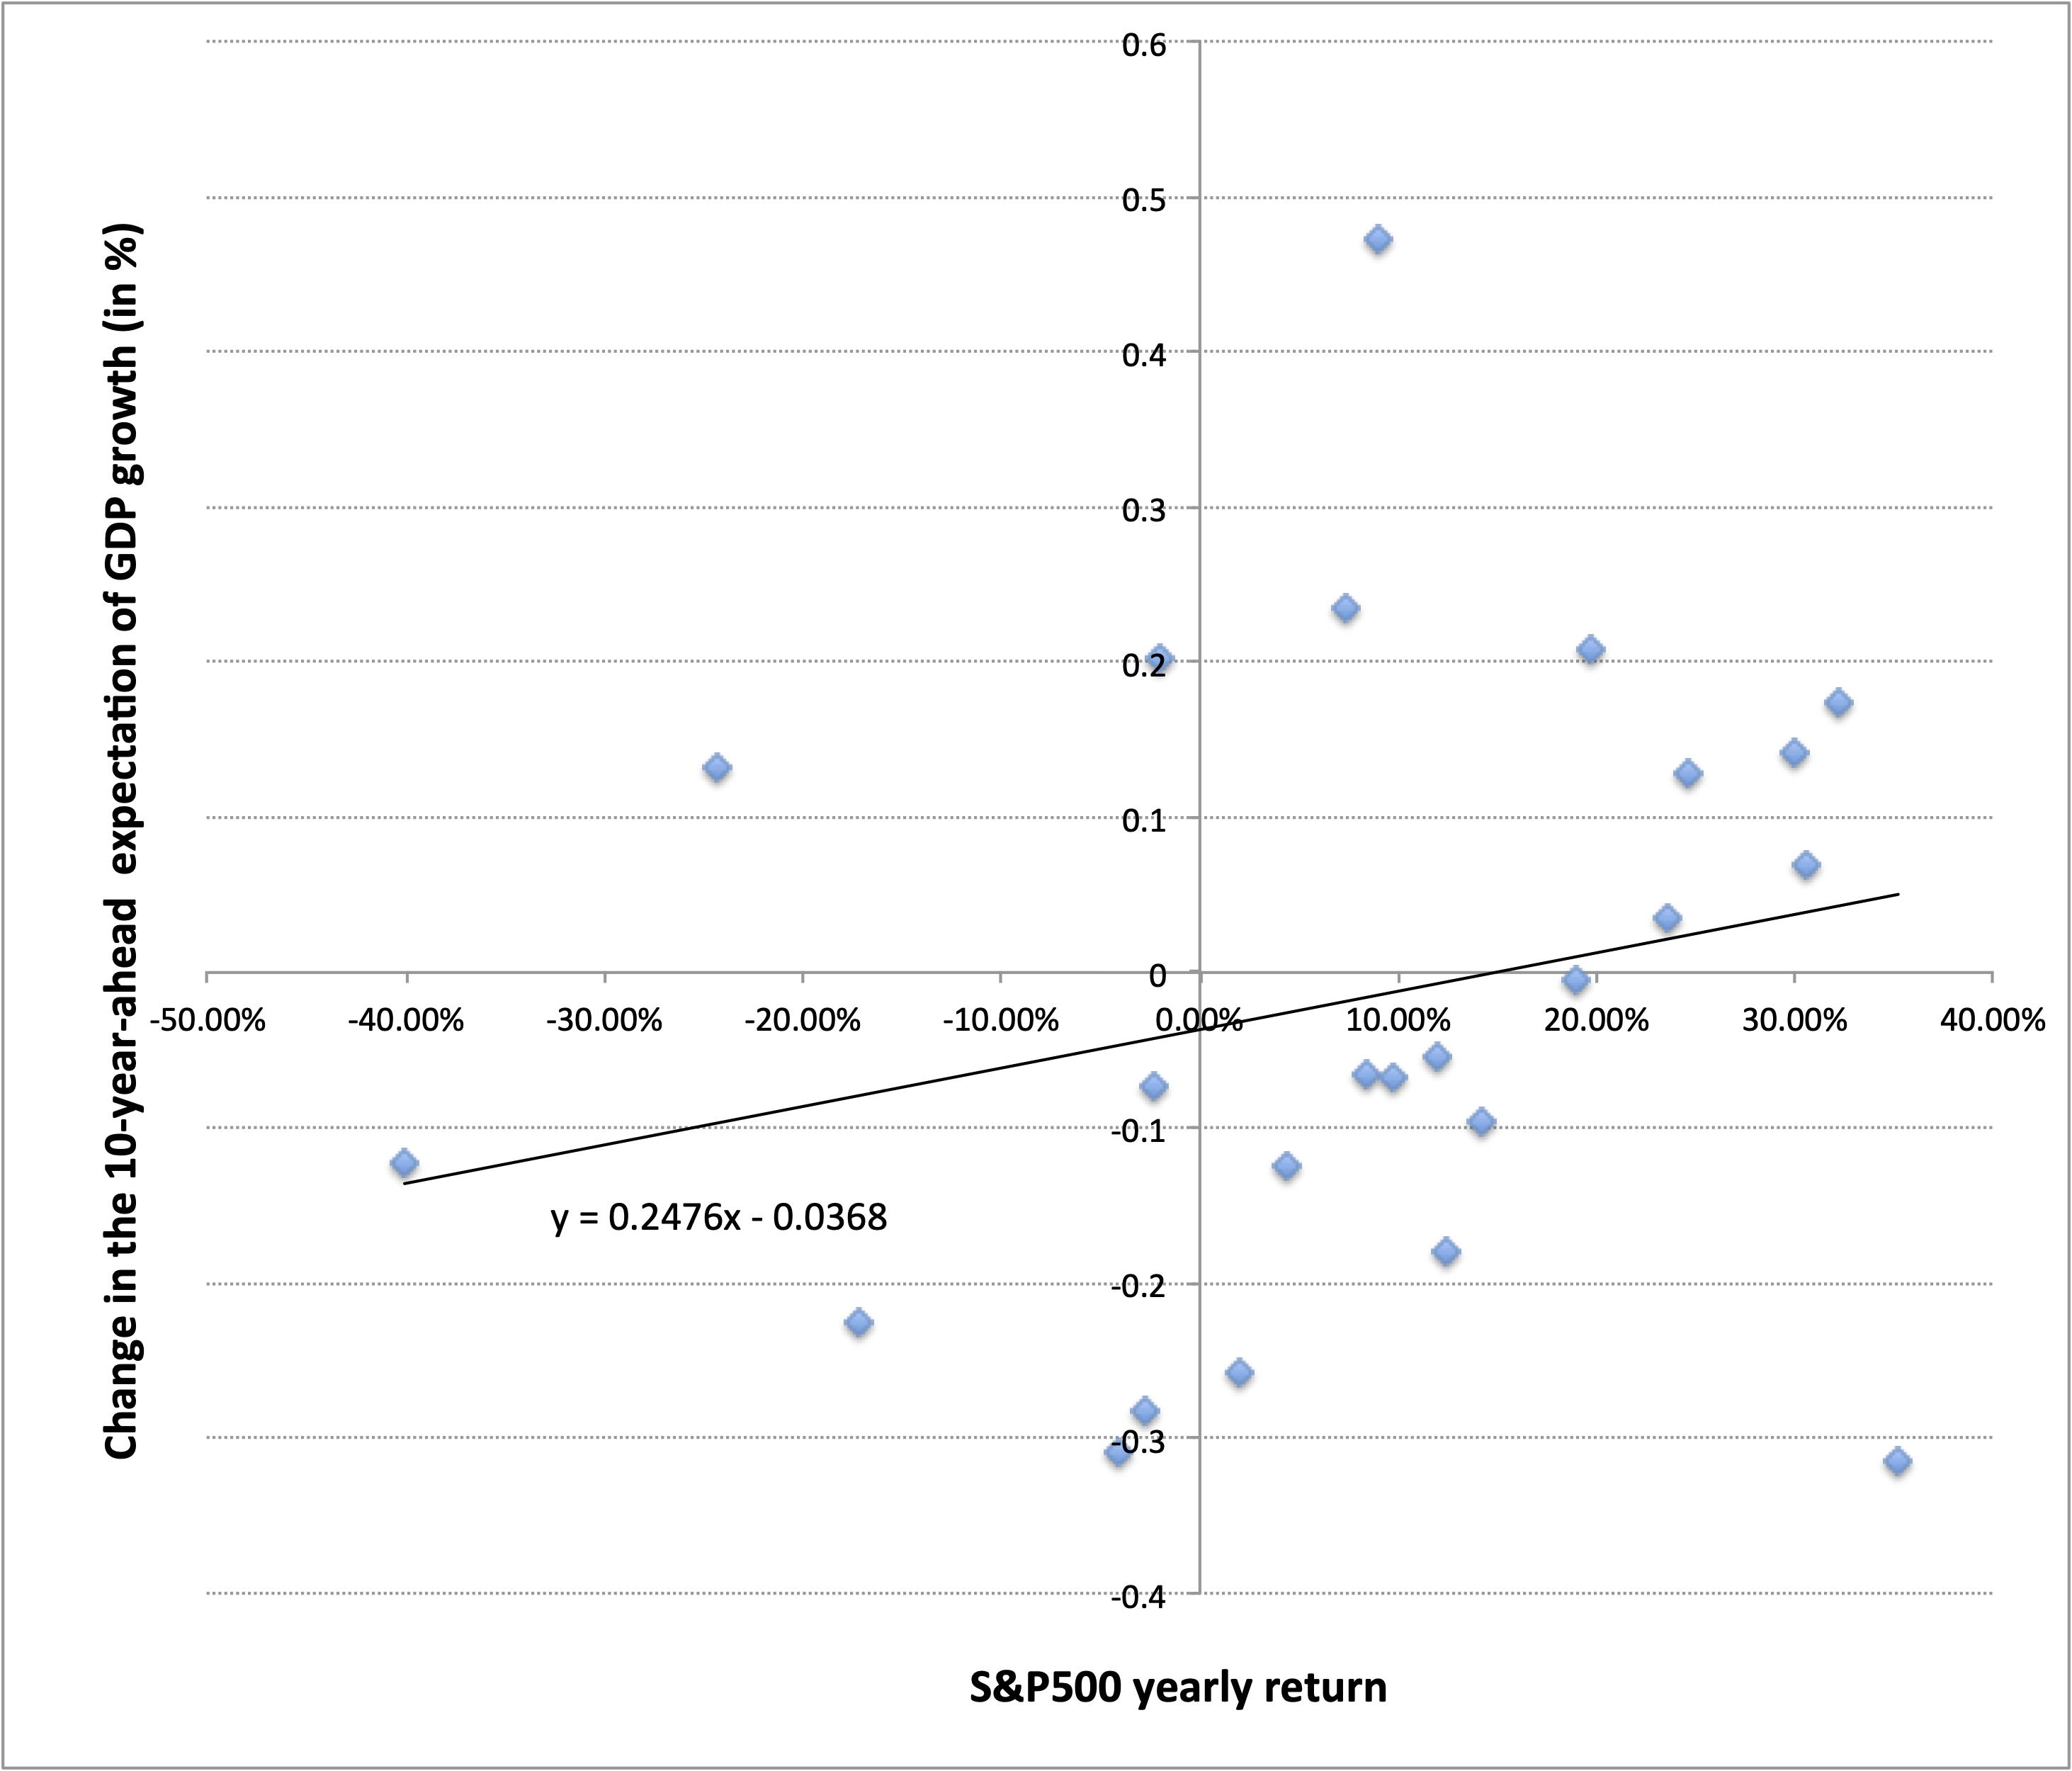
\includegraphics[width=.75\linewidth]{figures/Figure_Stock_chge_expect.pdf}
\end{figure}
\begin{scriptsize}

Source: \href{https://www.philadelphiafed.org/research-and-data/real-time-center/survey-of-professional-forecasters/data-files/rgdp10}{Philadelphia Fed S.P.F.}.
\end{scriptsize}
\end{center}
\end{frame}




